\begin{figure}[H]
  \centering
  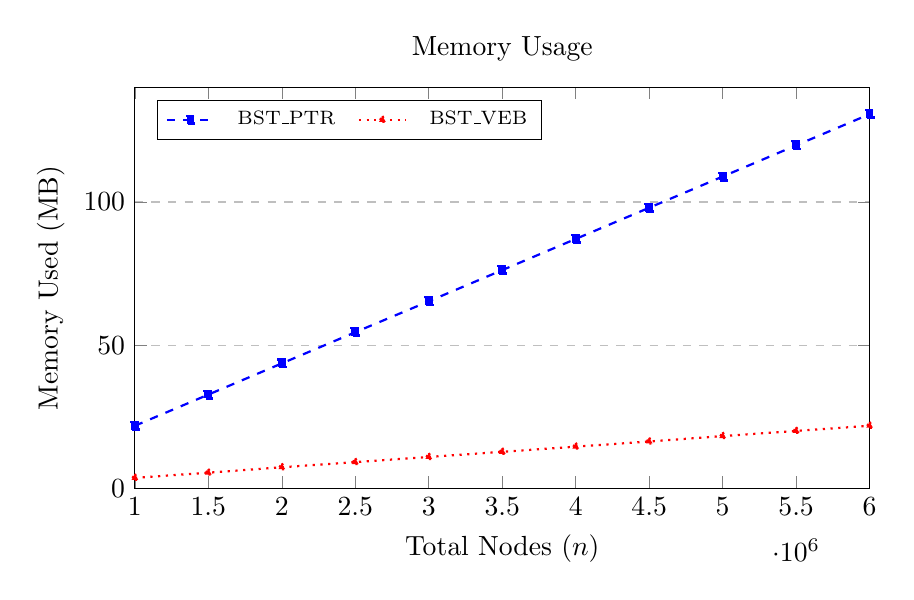
\begin{tikzpicture}
    \begin{axis}[
        title={Memory Usage},
        xlabel={Total Nodes ($n$)},
        ylabel={Memory Used (MB)},
        width=0.9\textwidth,
        height=0.55\textwidth,
        xmin=1000000, xmax=6000000,
        ymin=0, ymax=140,
        ymajorgrids,
        grid style=dashed,
        legend columns=2,
        legend pos=north west,
        legend style={font=\scriptsize, column sep=6pt},
    ]

    \addplot+[blue, thick, dashed, mark=square*, mark options={scale=.7,fill=blue}]
      coordinates {
        (1000000,21.8) (1500000,32.7) (2000000,43.6) (2500000,54.5)
        (3000000,65.3) (3500000,76.2) (4000000,87.1) (4500000,98.0)
        (5000000,108.9) (5500000,119.8) (6000000,130.7)
      };
    \addlegendentry{BST\_PTR}

    \addplot+[red, thick, dotted, mark=triangle*, mark options={scale=.7,fill=red}]
      coordinates {
        (1000000,3.6) (1500000,5.4) (2000000,7.3) (2500000,9.1)
        (3000000,10.9) (3500000,12.7) (4000000,14.5) (4500000,16.3)
        (5000000,18.2) (5500000,20.0) (6000000,21.8)
      };
    \addlegendentry{BST\_VEB}

    \end{axis}
  \end{tikzpicture}
  \caption{Memory usage in MB as a function of total nodes for the pointer-based (\texttt{BST\_PTR}) and VanEmde-Boas (\texttt{BST\_VEB}) implementations.}
  \label{fig:memorybig}
\end{figure}
